\subsection{Hyperparamters}

Through grid search the optimal combination of $\lambda$- and degree-values were found to be: 

\begin{table}[h!]
    \centering
    \begin{tabular}{|c|c|c|c|}
        \hline
        & & \textbf{Franke Function} & \textbf{Terrain Data} \\ \hline
        \textbf{Ridge} & $\lambda$ & 2.4 $\times 10^{-2}$ & 3.0 $\times 10^{-5}$ \\ 
         & degree & 7 & 4 \\ \hline
        \textbf{Lasso} & $\lambda$ & 1.7 $\times 10^{-5}$ & 2.2 $\times 10^{-4}$ \\ 
         & degree & 7 & 6 \\ \hline
    \end{tabular}
    \caption{Best pairs of $\lambda$- and degree values found through grid search}
    \label{tab:grid}
\end{table}

In the following sections, the Lasso and Ridge regression models are trained with their respective $\lambda$ values from Tab. \ref{tab:grid}. 

\subsection{Franke function}

\begin{figure}[h!]
    \centering
    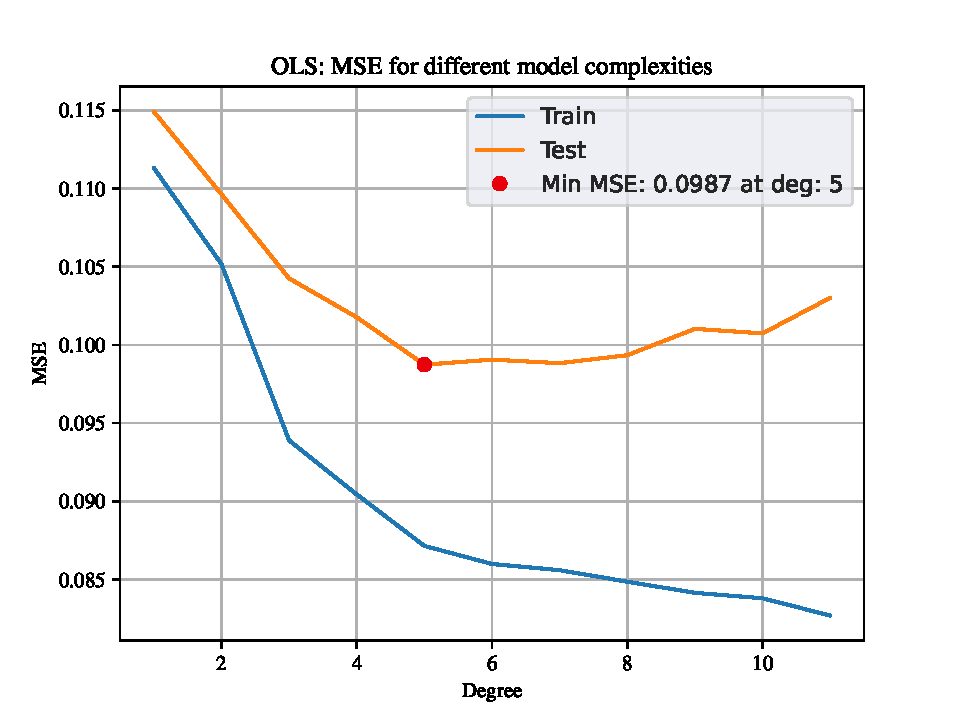
\includegraphics[width=1\linewidth]{project_1/figures/figures_in_report/OLS_MSE_Franke_Noise.pdf}
    \caption{Mean squared error (MSE) for the ordinary least squares model both on training- and test data. The minimum MSE is marked with a red dot. This displays the same concept as figure 2.11 in Hastie et.al. \citep[p. 38]{hastie}.}
    \label{fig:mseols}
\end{figure}

Fig. \ref{fig:mseols} shows how the mean square error (MSE) initially decreases as the polynomial degree increases. This seems reasonable as the Franke function makes up a complicated surface and higher degree polynomials are necessary to replicate it. 

Furthermore, we notice that the test error reaches its minimum at polynomial degree equal to 5. 
This minimum is chosen as the optimal polynomial degree. 
Beyond this point, the test error increases and the training error decreases.
This is due to overfitting, and the fact that OLS is designed to minimize the MSE of the training data. 

When the model is underfitted, i.e. a too low polynomial degree, we have high bias and low variance. At the other end however, when the polynomial degree is too large, the bias is low and the variance is high. 

\begin{figure}[h!]
    \centering
    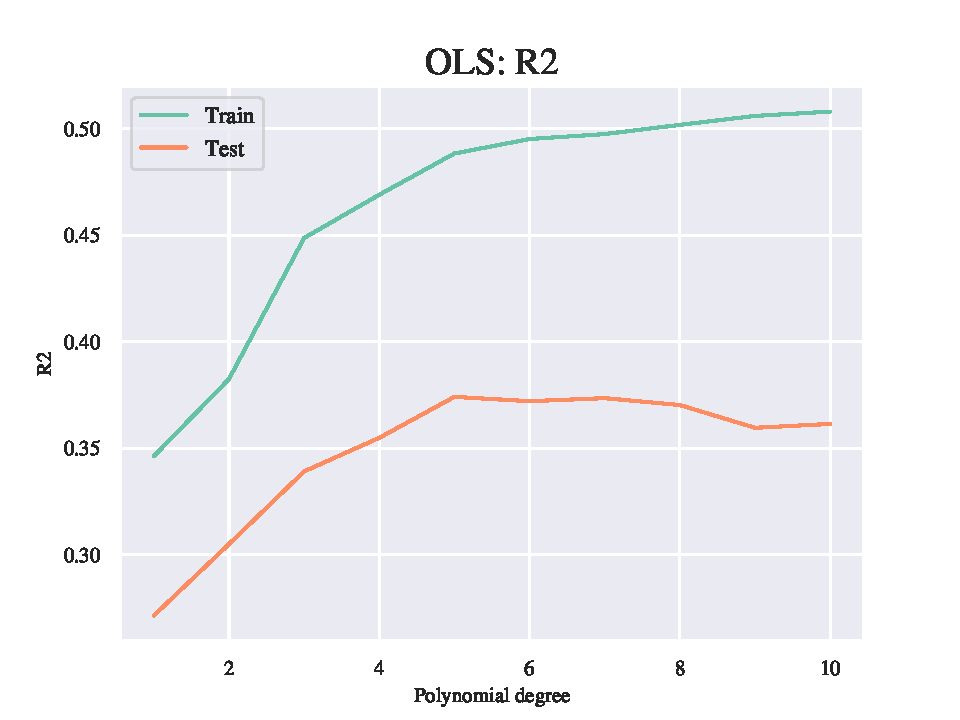
\includegraphics[width=1\linewidth]{project_1/figures/figures_in_report/OLS_R2_Franke_Noise.pdf}
    \caption{$R^2$ for the ordinary least squares model on training- and test data.}
    \label{fig:r2ols}
\end{figure}

As shown in Fig. \ref{fig:r2ols}, the $R^2$ value increases as higher degree polynomials are introduced to the ordinary least squares model. 
This is reasonable as we likely need higher degree polynomials to explain more variance in the data. The increase in $R^2$ halters at around degree equal to 10. 
At this point, introducing higher degree polynomials does not help explain further variance in the data. 
The value of $R^2$ for the test data is substantially lower then the one for the training data. 
This might be a sign that the model does not describe the underlying structure of the data precisely, in other words doesn't generalize well. 
This claim is further supported by an $R^2$ value of 0.50 on the training data, meaning that our model only explains 50 \% of the variance in the training data.
However, this is expected due to the large amount of noise we introduced in Eq. \ref{eq:franke_noise}.

\begin{figure}[h!]
    \centering
    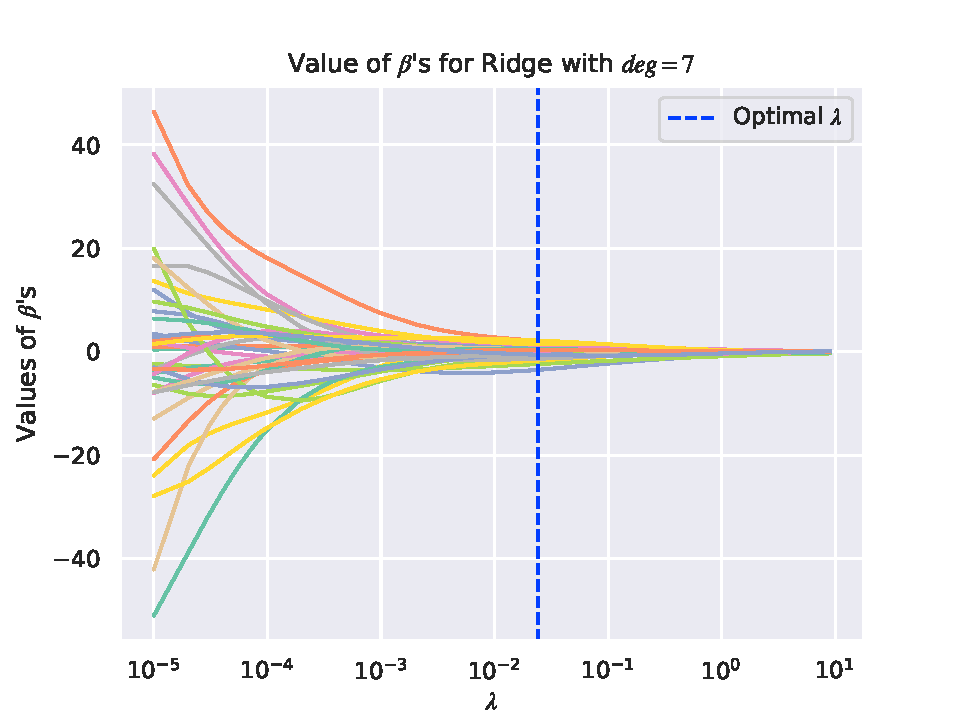
\includegraphics[width=1\linewidth]{project_1/figures/figures_in_report/Ridge_Betas_lambda_Franke_Noise_const_deg.pdf}
    \caption{The values of the parameters $\bet$ for the Ridge regression model with polynomials up to a degree of seven for increasing values of $\lambda$. Each colored line represents one $\beta_j$.}
    \label{fig:ridge_betas}
\end{figure}

\begin{figure}[h!]
    \centering
    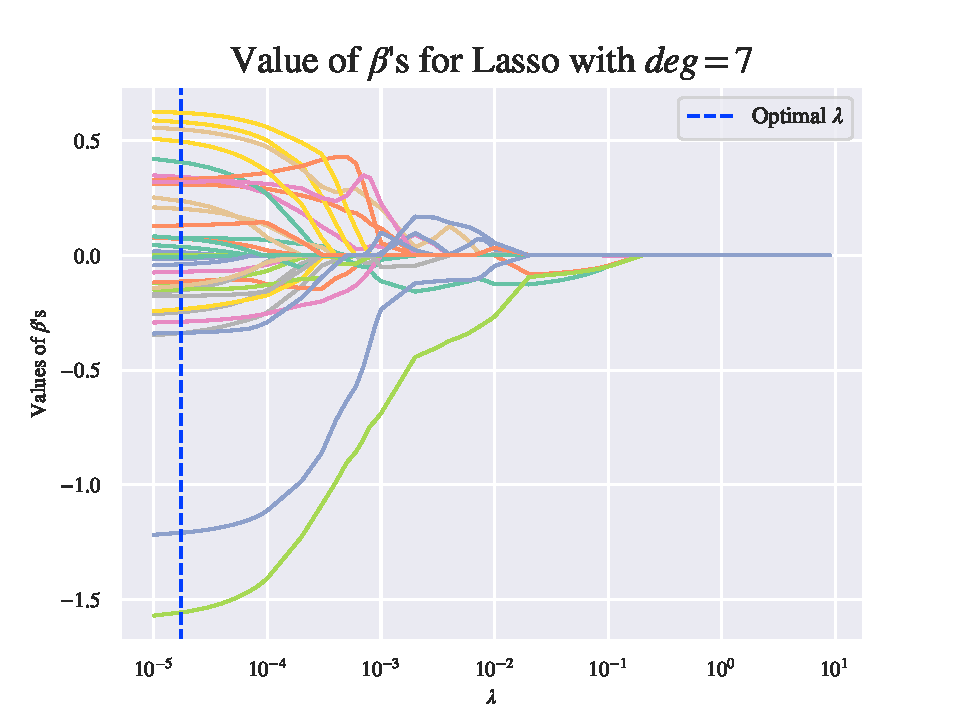
\includegraphics[width=1\linewidth]{project_1/figures/figures_in_report/lasso_Betas_lambda_Franke_Noise_const_deg.pdf}
    \caption{The values of the parameters $\bet$ for the Lasso regression model with polynomials up to a degree of seven for increasing values of $\lambda$. Each colored line represents one $\beta_j$.}
    \label{fig:lasso_betas}
\end{figure}

The $\bet$-values for our Ridge and Lasso regression models are presented in Fig. \ref{fig:ridge_betas} and Fig. \ref{fig:lasso_betas} respectively. 
For both models, we observe that the coefficients are forced towards zero as the penalty increases. 
For the Ridge regression coefficients, all have non-zero values regardless of the size of the penalty. 
For Lasso regression however, we observe that some are brought to zero at a sufficiently large penalty; 
closer to $\lambda = 10^0 = 1$ all values of the $\beta$'s are brought to zero. 
A $\lambda$ value of this size seems highly unreasonable, as it corresponds to a constant prediction, i.e. a flat plane normal to the $z$-axis.
The vertical line in each plot shows the optimal $\lambda$ in combination with the polynomial degree found through the grid search (numbers are available in Tab. \ref{tab:grid}). 
%This backs up the claim that $\lambda$'s higher than 1 seem unreasonable. 

We find it interesting that the Lasso regression model has a far lower optimal $\lambda$ value than the Ridge regression model.
However, we also note how the y-axis values in Fig. \ref{fig:ridge_betas} and in Fig. \ref{fig:lasso_betas} are different. 
Taking the latter into consideration, the beta values chosen for the final models are comparable. 

\begin{figure}[h!]
    \centering
    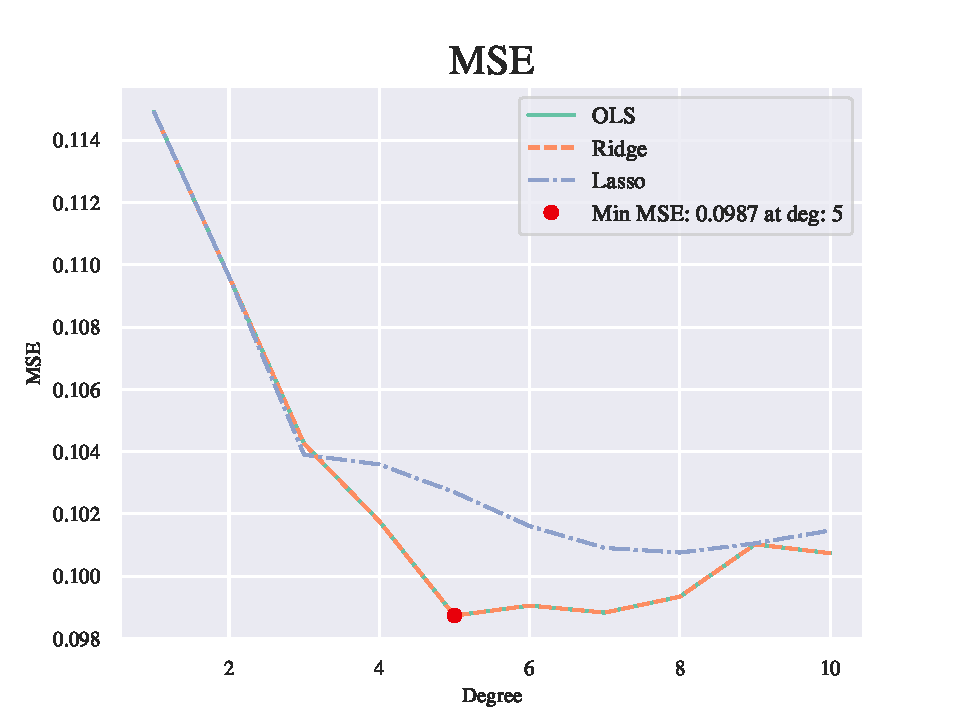
\includegraphics[width=1\linewidth]{project_1/figures/figures_in_report/OLS_Ridge_Lasso_Franke_Noise.pdf}
    \caption{The MSE on the test data for OLS, Ridge and Lasso regression models. The minimum MSE is marked with a red dot.}
    \label{all3franke}
\end{figure}

We want to find the best model among OLS, Ridge and Lasso regression. 
In Fig. \ref{all3franke} we see the MSE on the test data for all three. 
The best model on the Franke function data is OLS with a MSE of 0.0987. 
This is found at a polynomial degree of five.  

The Lasso regression model does not perform identically with OLS when $\lambda$ is set to zero. 
As fitting the Lasso model requires iterative tuning, we can not expect to reach the exact optimal $\beta$'s. 
For continuity, we decided on having a constant value for max iterations while fitting the Lasso models, at \texttt{max\_iter=1000}. 
Increasing this would result in a substantial increase in computation time for the grid search.
The Lasso regression model performs worse out of the three partly because it has not yet reached the optimal solution.

Furthermore, the Ridge regression model performs only slightly worse than OLS.
We suspect that the $\lambda$ value found through the grid search is not the optimal one, as a $\lambda$ value of $10^{-5}$ yield a lower minimal MSE for the test data. 
The cause of this is not apparent to us. 
Possible explanations might be that the grid search uses another train test split than the plotting files. 
This is to be able to run them separately, i.e. we don't want to have to run the relatively slow grid search every time we make a new plot.
To avoid this being a large source of errors, we use bootstrapping in the grid search. 
In this specific plot however, we only train on a simple train test split, which, if unlucky, can cause results that are not theoretically optimal.
At a closer inspection of different $\lambda$ values greater than zero for Fig. \ref{all3franke}, the Ridge regression model never outperforms OLS. 
The conclusion of OLS being the best model holds regardless. 

\begin{figure}
    \centering
    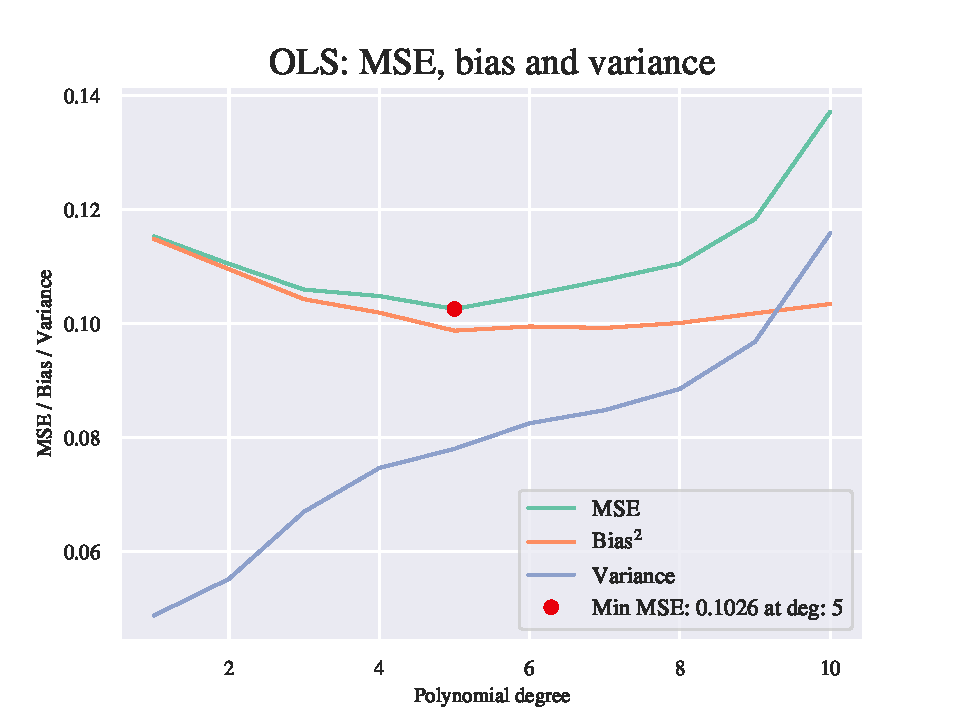
\includegraphics[width=1\linewidth]{project_1/figures/figures_in_report/bias_var_Franke_Noise_bootstrap.pdf}
    \caption{MSE decomposition in terms of bias and variance term for an ordinary least squares model trained with bootstrapping. The minimum MSE is marked with a red dot. 
}
    \label{bias_var_trade}
\end{figure}

With the use of bootstrap samples, we have calculated the MSE decomposed into a bias and a variance term for an OLS model. 
In Fig. \ref{bias_var_trade} the bias is initially high, but the variance is low. 
This is typical for an underfitted model. As the complexity increases, the bias goes down, whereas the variance increases. 
The lowest MSE is reached at some trade-off between the two. 
As the model complexity is further increased, the variance substantially increases and ensures an even higher MSE than at the beginning. 
This is a sign of an overfitted model.


\subsection{Terrain data}

\begin{figure}[h!]
    \centering
    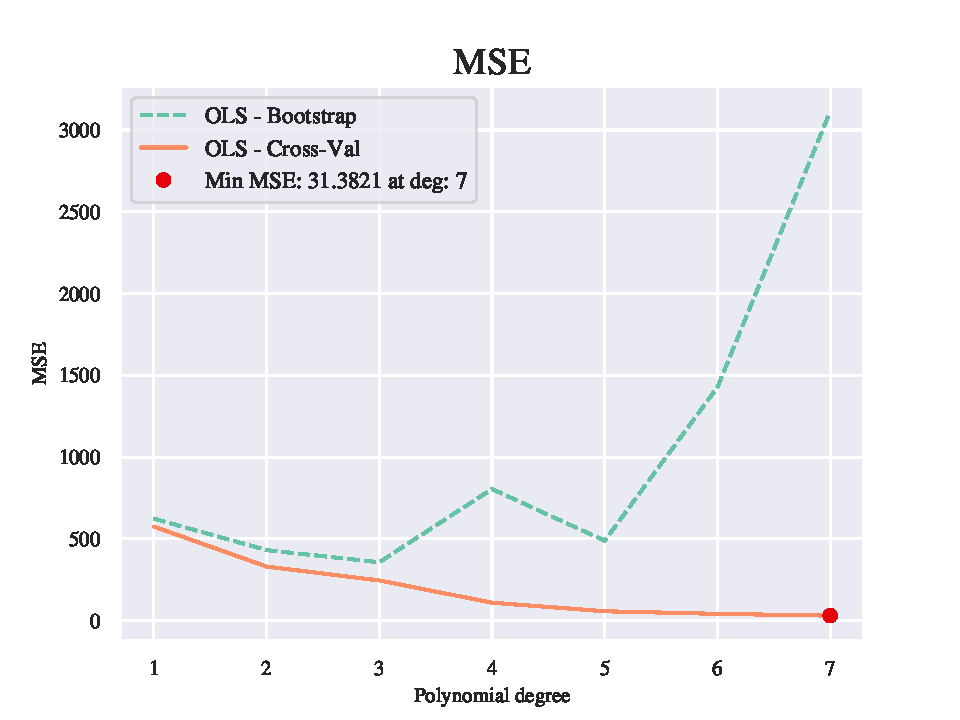
\includegraphics[width=1\linewidth]{project_1/figures/figures_in_report/CV_BS_OLS_terrain.pdf}
    \caption{MSE for OLS plotted against the polynomial degree, two different ways: 10-fold cross-validation and bootstrapping with 100 bootstrap samples. The minimum MSE is marked with a red dot.}
    \label{cv_versus_bs}
\end{figure}

In Fig. \ref{cv_versus_bs} we compare bootstrapping to cross-validation. 
Both resampling techniques are used on the ordinary least squares model. 
The minimal MSE value for the cross-validated OLS model is lower than for the bootstrapped model. 
%We do not plot higher polynomial degrees as we then reach problems with numerical precision (numbers lower than $\approx 10^{-15}$) and the MSE wrongly increases quickly.  

There might be several reasons why the MSE is lower for cross-validation compared to bootstrapping. 
For the model trained with cross-validation, more data is utilized than for the one trained with bootstrap. 
In the latter, we split into a training and a test data set, whereas cross-validation trains on the entire data set.
Indeed, as we use an 80/20 train-test split, and bootstrap on average uses 63.2\% of the train data each sample, the bootstrap ends up using only 50.6\% ($0.8\cdot 63.2\%$) of the training data on average \citep[p. 251]{hastie}. 
Compared to 10 folds cross validation, which uses 90\% of the data for training each fold, it is expected that the bootstrap model will overfit at a much lower complexity.
 
We could have used the entire data set to draw bootstrap samples from, which would have allowed us to use more data.
However we would then have to keep track of which samples were not included in the bootstrap sample and use these as the test set for the specific bootstrap model. 
This was not done, as it would have required us to implement bootstrapping twice for the different purposes in this report.

For the cross-validated model we tried different number of folds in the range 5 to 10. 
The results were very similar, with $k = 10$ giving the lowest MSE. 
Seeing as computing power was not an issue in this part, we chose k = 10 as our final value. 
This is used for all bootstrapped models for the terrain data.

\begin{figure}[h!]
    \centering
    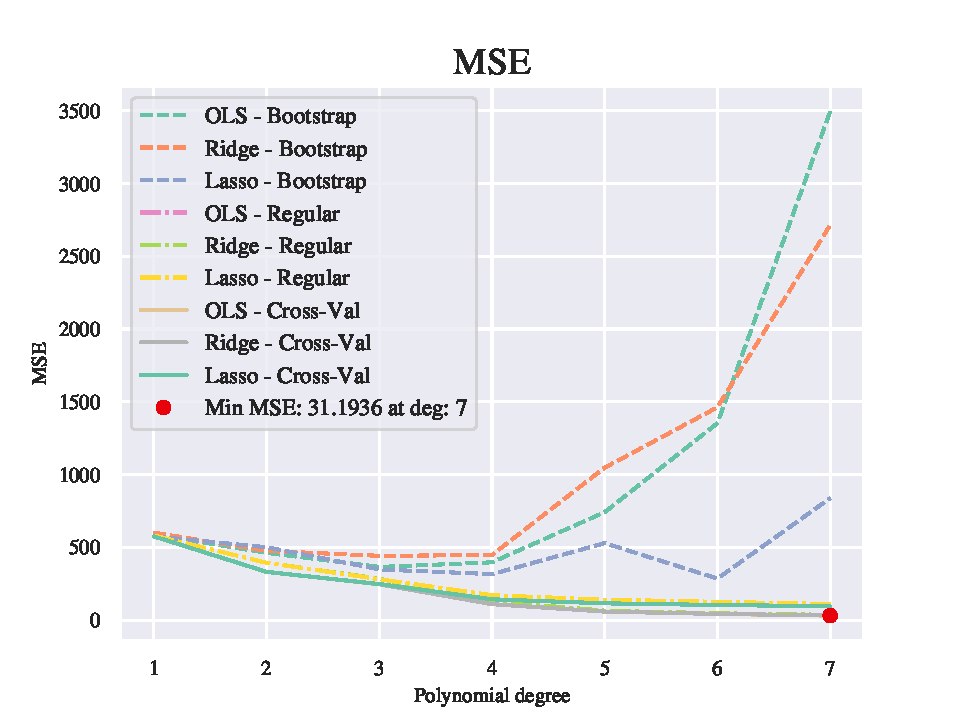
\includegraphics[width=1\linewidth]{project_1/figures/figures_in_report/All_terrain.pdf}
    \caption{MSE for OLS, Ridge and Lasso regression against polynomial degree. Each model is trained three times; with no resampling, using 10-fold cross-validation and lastly, using bootstrapping with 100 bootstrap samples. The minimum MSE is marked with a red dot.}
    \label{all_terrain}
\end{figure}

Our main goal is to find the model providing the best fit, with respect to the MSE, for the terrain data.
We have implemented three different model types; OLS, Ridge, and Lasso. 
Furthermore, we can use no resampling, bootstrapping or cross-validation. 
Combining this yields nine different models. In Fig. \ref{all_terrain} we compare the MSE on the test set for all. 
We find OLS with 10-fold cross-validation to be the best model, with a MSE value of 17.6863 at a polynomial degree of 10.
This plot is only created for degrees of complexity up to 11 seeing as there are problems with numerical precision beyond this point (numbers smaller than $\approx 10^{-15}$).
The bootstrapped models are excluded from the plot beyond a polynomial degree of seven, as including them would dominate the visualization.

We believe that 10-fold cross-validation is performing best, as it combines being trained on the most data (90\% of the data each fold), while also being trained multiple times. 
This results in a more stable model, that handles new test sets better than any other.
It is possible that cross-validation with more than 10 folds would have performed even better, however we avoided this due to it requiring more computational power.
Even though it would be feasible to train it on data sets of this size, it would not be well generalizable for larger data sets.

Choosing the number of data points for the terrain data was challenging. Including more data points meant having a data set with more variance. This leads to models with a far higher MSE. 
Another aspect we considered was the computational time. Especially the grid search is already time consuming with 1681 data points. 

%Further work to do on this could include a different implementation of the bootstrap method.

Furthermore, it is interesting to discuss whether linear models are sufficient for these kinds of problems or not. Intuitively one might think that more complex is better, and that the only downside of more complex models are computational efficiency. While being more computationally efficient is definitely an advantage that should not be neglected for large quantities of data, it's far from the only upside of these simpler models. 
 
Firstly, linear models generally propose more explicit relationships, i.e. they're easier to interpret. To what extent different feature-variables affect the response-variable is simply stated by the slope's relation to the corresponding parameters, and can thus be deferred straight from the coefficients. The explainability of a model is crucial for justifying the use of analytical and predictive models in close to all real-world problems. 

Secondly, and maybe most obviously, if the true relationship we're trying to model is actually linear (or approximately so) - a linear model will be ideal for trying to mimic this relationship. While some more complex models might be able to imitate this performance, there is no reason to use overly complicated methods that increase the risk of overfitting, reduce the interpretability and are more computationally heavy. 